%! Author = adnansiddiquei
%! Date = 07/12/2023

\section{Development, Experimentation and Profiling}\label{sec:development-experimentation-and-profiling}
Here we discuss several components of the development process, and reason why we chose to do things in certain ways

\subsection{Linting and Formatting - \inlinecode{ruff}}\label{subsec:linting-and-formatting}
    Linting and formatting is useful, especially in shared projects, as it allows for a consistent style across the codebase.
    There are a plethora of python linting and formatting tools available and for this project, we chose to use \inlinecode{ruff}.
    There were two primary reasons for this choice: speed and simplicity.
    \inlinecode{ruff} is faster than most other linting tools including \inlinecode{flake8}.
    In a test done by the developers of \inlinecode{ruff}, it managed to lint the CPython codebase 42x faster than
    \inlinecode{flake8} \cite{ruff-repo}.
    Whilst speed of linting is not a primary concern for this project, it doesn't hurt to pick the faster option.

    Additionally, \inlinecode{ruff} provides formatting functionality and as such it can also replace tools such as
    \inlinecode{black}.
    This makes the implementation of linting and formatting simpler, as we only need to use one tool.
    \inlinecode{ruff}'s configuration capabilities allow it to lint and format to any standard we want to, and as such,
    it was configured to mimic \inlinecode{black} and \inlinecode{flake8}'s default config in accordance with PEP8.

    \subsection{Git and Gitlab Workflows}\label{subsec:git-and-gitlab-pipeline}
    It is generally good practise to write detailed commit messages and merge requests, and traditionally in larger
    software projects, project management tools such as JIRA are used to track issues and tasks, and merge requests
    are linked to these issues.
    In the world of open source, and small projects like this, GitLab's issue tracker works as a perfect tool for this.
    Therefore, we utilised the issue tracker to create issues for tasks that needed to be done, and then linked merge requests
    to these issues.
    In this way, we could maintain detailed documentation in the issue tracker of what was done, and why it was done,
    in a slightly more structured way than just using commit messages.
    Therefore, a new branch was created for every issue, and once the branch implemented or resolved the features in the
    issue, a merge request was created, linked to the issue, merged into main, and the issue was closed.
    As such, anyone with access to the repo can see the git commit history through the GitLab UI and any references to issue
    numbers in commits can be clicked to link the user to the underlying issue which describes what was implemented and why.

    Furthermore, a nice feature of many project management tools and IDE's is the ability to group branches into folders
    based on the branch name.
    Git allows forward slashes '/' in branch names such that branches can be structured into folders by the IDE, as such
    a naming convention was adopted for branches.
    Branches were named like the following: \inlinecode{feat/issue-1} or \inlinecode{tests/issue-4} where the 3 main
    'folders' used were \inlinecode{feat} for feature, \inlinecode{tests} and \inlinecode{bug}, followed by
    the issue number it implemented.
    In practise, the \inlinecode{bug} folder was not used as bugs as no bugs were discovered.
    Occasionally a \inlinecode{report} branch was created when only the report needed to be updated, these were not linked
    to any issues.

    Overall, these Git and GitLab workflows allowed for a structured development process, and a detailed history of
    what was done and why it was done, which is useful for future reference.

    \subsection{Test Driven Development}\label{subsec:test-driven-development}
    Where possible, we strived to do test driven development by writing tests first.
    This was made possible due to the careful prototyping and API design discussed in Section\eqref{sec:solution-design}.
    The reason we decided to write tests first came from three primary reasons:
    \begin{itemize}
        \item it streamlined code writing, as we were already aware of what the code needed to do, and what the edge cases
        were.
        \item it defined clearly what the end product would be;
        \item it reduced debugging time.
        We could more quickly figure out what was going wrong if a bug arose;
    \end{itemize}
    The final tests that were written are discussed more in Section\eqref{sec:validation-unit-tests-and-ci-set-up}.

    \subsection{Profiling and Optimisation [TODO]}\label{subsec:profiling-and-optimisation}
    \begin{figure}[htb]
    \centering
    \begin{subfigure}[b]{0.9\linewidth}
        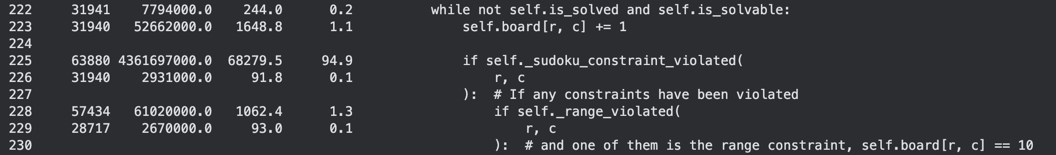
\includegraphics[width=\linewidth]{figures/line_profile1}
        \caption{An excerpt of the line profile of the \inlinecode{Backtracking().solve} function. Line 220 indicates
        the that the \inlinecode{Backtracking()._sudoku_constraint_violated} function consumes the vast majority of the
        computation time.}
    \end{subfigure}
    \hfill
    \begin{subfigure}[b]{0.9\linewidth}
        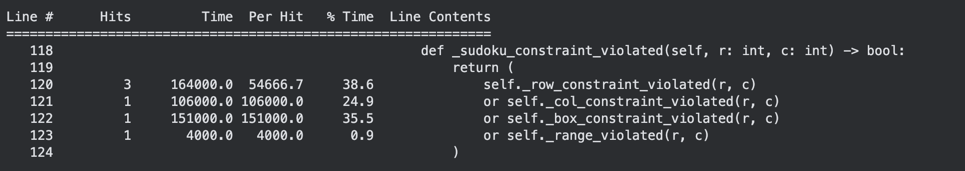
\includegraphics[width=\linewidth]{figures/line_profile2}
        \caption{The line profile of the \inlinecode{Backtracking()._sudoku_constraint_violated} function. This indicates
        that no single line of code is responsible for the majority of the computation time.}
    \end{subfigure}
    \caption{Line profiles of the \inlinecode{Backtracking().solve} function and the
    \inlinecode{Backtracking()._sudoku_constraint_violated} functions. The headers of each column are shown in (b).}
    \label{fig:line_profile}
    \end{figure}
    Given that this was a very low requirement project, there was not much testing of third-party packages required.
    However, the performance of the code was tested using a line profiler.
    Fig.\eqref{fig:line_profile} shows the line profile of the \inlinecode{Backtracking().solve} function, which allowed
    us to identify the bottleneck of the code, where most of the time was being spent.
    This is useful as it allows us to identify where to focus our optimisation efforts, and not waste time optimising
    code that is not responsible for the majority of the computation time.

    Given that \inlinecode{Backtracking()._sudoku_constraint_violated} was the function that we identified as the
    bottleneck, the next steps would be to optimise this function.
    Some options for this would be to re-write this function in Cython or C, or look into different algorithms / packages
    that could be used to implement this function.
    This was not done for this project but this section is included to illustrate the importance of profiling before
    optimisation.

    \subsection{Coding Best Practises [TODO]}\label{subsec:coding-best-practises}
    Modularisation.
    typing.
    Exceptions. Error handling, try except. Never catch all exceptions.
